\documentclass[12pt]{article}

\usepackage{sbc-template}
\usepackage{amsmath}
\usepackage{graphicx,url}

\usepackage[english]{babel}   
%\usepackage[latin1]{inputenc}  
\usepackage[utf8]{inputenc}  
% UTF-8 encoding is recommended by ShareLaTex
\usepackage{verbatim}
\usepackage{listings}
\usepackage{xcolor}

\definecolor{verde}{rgb}{0,0.5,0}

%para customizar o código (ver https://en.wikibooks.org/wiki/LaTeX/Source_Code_Listings)
\lstset{language=Python, %defina a linguagem usada no trabalho
              belowcaptionskip=1\baselineskip,
                breaklines=true,
                frame=false,
                xleftmargin=\parindent,
                showstringspaces=false,
                basicstyle=\footnotesize\ttfamily,
                keywordstyle=\bfseries\color{green!40!black},
                commentstyle=\itshape\color{purple!40!black},
                identifierstyle=\color{blue},
                stringstyle=\color{orange},
                numbers=left,
            }

\sloppy

\title{Deep Learning - A brief study of Main Approaches and Architectures}

\author{Bryan Mauricio Reinoso Cevallos}


\address{Student from Burgos's Polytechnic School
  \email{brc0007@alu.ubu.es; cevallos.reinoso10@e-uvt.ro}
}

\begin{document} 

\maketitle
\begin{abstract} 
  The main goal of this paper is to do a brief study and comparison of main architectures of Deep Learning.
  
  Firstly, a state of the art chapter is goin to be presented where I am going to do a brief introduction to the Deep Learning. Because this paper is about a very dificult subject, a deep state of the art is almost impossible to do in 6 to 12 pages, so in this first chapter is going to be a brief introduction of the main topic and the differents main approaches of this matter.
  
  Secondly, a more detailed chapter with the main architectures is going to be presented. Also, some problems and models are going to be written in this chapter.
  
  Thirdly, I am going to write a deep report about the application made by my classmate and me and the result we obtained. This application is going to be explained in detail. Also, a report of the results is going to be presented.
  
  Lastly, a chapter with some conclusions and future work in this topic.
  
  \textbf{Keywords}: Deep Learning.
\end{abstract}

\section{Introduction: State of the art}

Firstly, in order to understand the main purpose of this topic, we also have to understand why Deep Learning is called that and what kind of problems are going to be addressed in this field.

So, We have to understand that when we talk of Deep Learning, we are talking of a field which address very complex problems. In order to solve this kind of problems a knowledge representation is needed. This representation is based in the real world knowledge and its purpose is to be understandable by the computer. Then, we are going to be able to build some architectures and algorithms to address these problems under this representation.

Therefore, this representation will allow us to model the problem and the training examples. The training examples are a representation of the problem in a particular case and, if we are talking of supervised training, a label with the solution of the problem for that particular case.With this training examples under the representation, we have the codified knowledge to build the algorith and the architecture which is going to learn from that information.

Because this information represents the knowledge of a specific task, we can say that we need a deep model that can capture the information of the problem under its representation and build a complex function with which to generalize the knowledge provided by the training examples.

Thus, in order to address these problems to achieve acceptable results, researchers began to model better and deeper algorithms and architectures of which major ones are going to be presented.

\subsection{Neural Networks}
One of the most popular models for Deep and Machine Learning. Because this is the method used for the application its presentation is going to be described in one section below (See Section \ref{sec:Neural Networks}).

\subsection{Boltzmann Machines}

\subsection{Other honorable mentions}
After the presentation of Boltzmann Machines and Neural Networks, I think is interesting to present another three algorithms that are also powerful and could be used to solve complex problems.

\subsubsection{Linear Regression}
Linear Regression is one of the mos used algorithms to predict a certain value or to classify from a serie of features that represent every input example. The intuition of this process is to draw a line through the examples which minimize the cost function. In order to understand this intuintion we can see the Figure \ref{fig:figure3}.

\begin{figure}[ht]
\centering
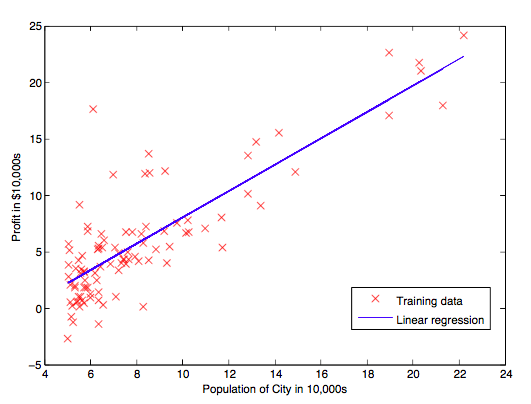
\includegraphics[width=.4\textwidth]{Regression.png}
\caption{Linear Regression}
\label{fig:figure3}
\end{figure}

So, in this algorithm we have two principal components. One is the cost function whose minimization is the objetive of Linear Regression. The second one is the hypotesis which is a linear function that represents the line to be drawn whose components are the $\theta$ value. 

Firstly, the cost functions is defined by the sum of the quadratic difference between the hypotesis and the objetive value of all training examples:

\begin{equation}
  J(\theta)=\frac{1}{2m} \displaystyle\sum_{i=1}^{m} (h_{\theta}(x^{(i)})-y^{(i)})^2
\end{equation}

Secondly, the hypotesis that is only a equation for a line but with the $\theta$ value that is going to change in the training in order to get the best fit for the data.

\begin{equation}
  h_{\theta}(x)=\theta^Tx=\theta_{0}+\theta_{1}x_{1}
\end{equation}

And this is Linear Regression algorithm which consist in draw the straight line through the training examples that minimize the cost function. Now, to obtain the best value $\theta$ for the problem, we have to use another algorithm and the most popular is Gradient Descent. And, in particular, we are going to present Batch Gradien Descent (see Section \ref{sec:Gradient}).

\subsubsection{Logistic Regression}
Logistic Regression has almost the same intuition as Linear Regression but in this case we are not trying to draw a straight line but a curve (See Figure \ref{fig:figure4}).
\begin{figure}[ht]
\centering
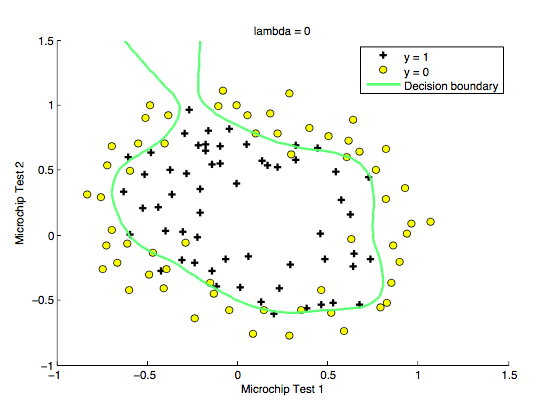
\includegraphics[width=.6\textwidth]{Logistic.png}
\caption{Logistic Regression}
\label{fig:figure4}
\end{figure}
Also, Logistic Regression algorith has two components in its process to obtain the best curve to fit the data.

The first one is the cost function. The formula of the cost function for Logistic Regression seems harder than the formula for Linear Regression, but it is only the logarithmic function of the hypotesis or one minus the hypotesis dependind if the expected value is one or cero. So if the expected value is cero, then the cost function for that example is the logarithmic funtcion of one minus the hypotesis for that example, and, if the expected value is one, the cost functions is the logarithmic function of the hypotesis. The total cost function is the sum of the cost functions of all training examples. The formula is:
\begin{equation}
  J(\theta)=\frac{1}{m} \displaystyle\sum_{i=1}^{m} [-y^{(i)}\log(h_{\theta}(x^{(i)}))-(1-y^{(i)})\log(1 -h_{\theta}(x^{(i)}))]
\end{equation}
 The intuition for the formula is that, when you are trying to predict one, if the hypotesis is close to one the algorithmic function will return a number close to cero. And, if you are trying to predict cero, when the hyposetis is close to cero, we subtract a lower amount from the one value and we are requesting the logarithmic function value for a number close to one that is cero. So, when we are far from the expected value, the cost funciont is going to be higher.
 
 Now, the second component, is the hypotesis. Unlike in Linear Regression, in this algorithm we are trying to draw a curve that fits the data, so, the hypotesis is going to be a nonlinear function. In this case we are talking about the sigmoid function.
 
 \begin{equation}
  h_{\theta}(x)=g(\theta^Tx)=\frac{1}{1+e^{-\theta^Tx}}
\end{equation}

 And, like in Linear Regression, to calculate the $\theta$ value we have to perform an update for the $\theta$ using another algorith. This algorith can also be the Batch Gradient Descent (see Section \ref{sec:Gradient}).
\subsubsection{Batch Gradient Descent}
\label{sec:Gradient}
Batch Gradient Descent is an algorith that determines the way we perform an update of the theta values. In every iteration of the training an uptdate is going to be performed. In Batch Gradien Descent we use all training examples to calculate the update needed to be performed. 

So, in each iteration of the algorith, batch gradient descent is going to perform the update:

 \begin{equation}
 \theta_{j}:= \theta_{j} - \alpha \frac{1}{m} \displaystyle\sum_{i=1}^{m} (h_{\theta}(x^{(i)})-y^{(i)})x_{j}^{(i)}
\end{equation}

We have to know that this update is done simultaneously in $\theta_{j}$ for all $j$. With this update our $\theta$ parameter come closer to the optimal and, in result, our cost function $J(\theta)$ decrease achieving the lowest cost.

In order to increase the performance of the algorithm, it is common to use the gradient values. these gradients are calculated at the same time as the cost function increasing the overall performance.

\begin{equation}
 \frac{\partial J(\theta)}{\partial\theta_{j}}= \frac{1}{m} \displaystyle\sum_{i=1}^{m} (h_{\theta}(x^{(i)})-y^{(i)})x_{j}^{(i)}
\end{equation}

It is noteworthy that there are some other updating algorithms to increase more the performance.
\section{Model used in the application: Neural Networks} \label{sec:Neural Networks}
It is well known that when we speak of Machine Learning and Deep Learning, one of the most widespread models are Neural Networks. Neural Networks, as you probably know, are a model based on the biological structure of brain neurons and their interconnection.

With this model, we are able to build some neural networks capable of learning complex nonlinear functions. These functions are an abstraction of the knowledge extracted from the training examples. With this complex nonlinear function we should be able to generalize knowledge to other new examples never seen by the neural network.

Neural Networks are composed of artificial neurons, which have an activation function, a series of inputs and an output. The process that this neuron does is to receive these inputs, and each input has a weight that will multiply with it. After this, a summation is made between all the previous results. This summation is given to the activation function that will return the output of the neuron. And, because the Neural Network has several neurons, it can abstract the complex nonlinear funcions which is composed by all calculations that every neuron do. An illustrated example of this operation can be seen in the Figure \ref{fig:figure1}.

\begin{figure}[ht]
\centering
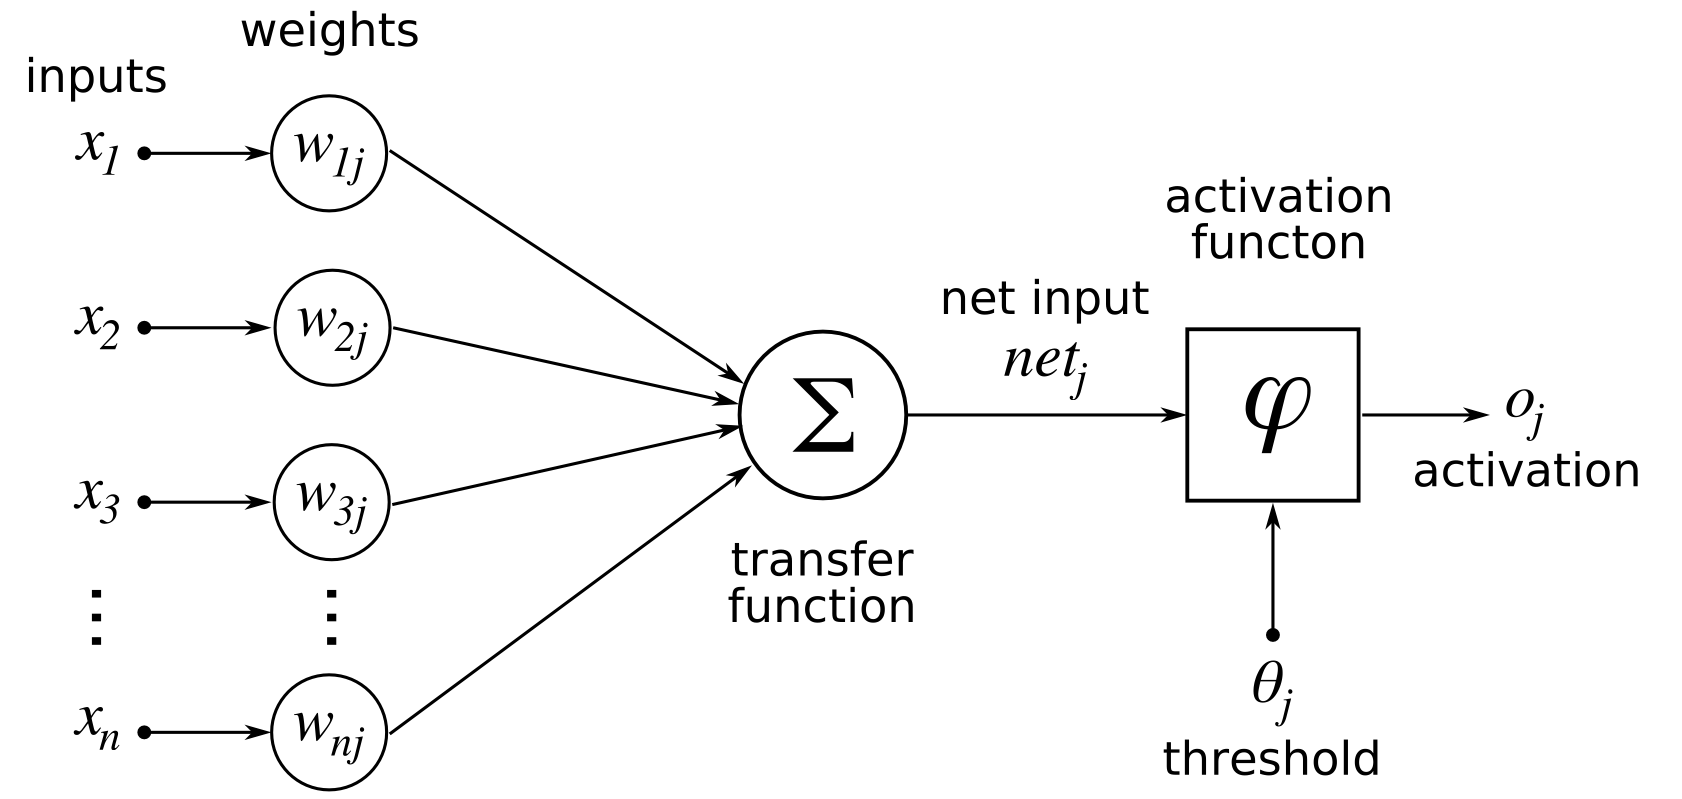
\includegraphics[width=.6\textwidth]{Neuron.png}
\caption{Artificial Neuron}
\label{fig:figure1}
\end{figure}

Knowing how artificial neurons works, we have to know how this neurons are organized inside the neural network. The neural network architecture is divided in, at least, two layers. One layer is called input layer, and the other one is called ouput layer. And, between this two layers, we can add one or more hidden layers. Of course we have to hae in mind that the bigger the numer of layers is, the more calculations and training complexity we have. We can se an example of a neural network with multiple layers in Figure \ref{fig:figure2}. Also, we have to think of the possibilitie of concatenate neural networks in order to solve more difficult problems or to build a better pipeline for the problem.

\begin{figure}[ht]
\centering
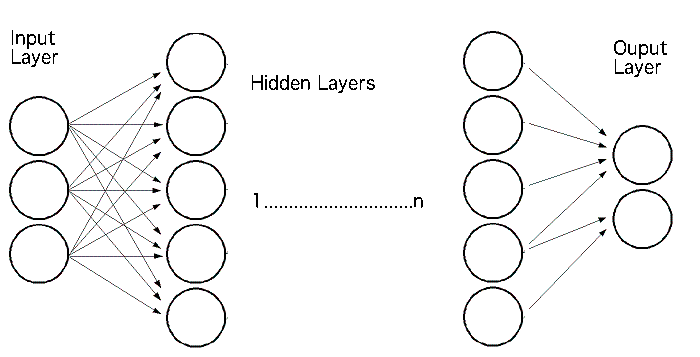
\includegraphics[width=.6\textwidth]{network.png}
\caption{Artificial Neuron}
\label{fig:figure2}
\end{figure}

Now, the matter is how a Neural Network can abstract the knowledge from the problems. The answer lies in the representation of the problem and, more specifically, in how we tune this model. So, firstly, we, as Deep Learning Engineers, must build a good representation of the problem for being understood by the computer. And lastly, we shloud tune the Neural Network in order to obtain the best results. This can be done by changing the number of layers, the way the layers are interconnected, the activation functions of the neurons, the restrictions of the supervised training, etc... Of course this procces of tunning is not easy, we can't be sure which configuration is going to work best and there is not a way to predict this.

Neural Networks have a lot of applications which the main ones are Character and Image recongnition, Image Compression, Stock Market Prediction and Some medicine applications such as cancer prediction.
\subsubsection{Multilayer}

\section{Description of the application and its resuslts}

There are three main components to be described in this section. The first one is the architecture and tool used and developed for this application. The second one is the data used to train the model and to test it. And, the last one, is the results obtained while and afteher the training of the Neural Network.

\subsection{Architecture and tool}

Firstly, we choose the Theano tool because is one of the most popular tools and is for Python which is a very malleable and easy used.

\subsection{Dataset Used: Heart Disease Data Set \cite{Lichman:2013}}

\subsection{Results}

\section{Conclusion}

\bibliography{sbc-template}
\bibliographystyle{plain}

\end{document}
